% ------------------------------------------------------------------
\renewcommand{\thisweek}{MATH327 Week 3}
\renewcommand{\moddate}{Last modified 15 Feb.~2021}
\setcounter{section}{3}
\setcounter{subsection}{0}
\phantomsection
\addcontentsline{toc}{section}{Week 3: Canonical ensemble}
\section*{Week 3: Canonical ensemble}

\subsection{The thermal reservoir}
\subsubsection{Replicas and occupation numbers}
While it is relatively easy to prevent particle exchange, for example by sealing gases inside airtight containers, it is not practical to forbid energy exchange as would be needed to fully isolate statistical systems.
Any thermal insulator is imperfect, and even in the deepest reaches of space we would still be bombarded by cosmic microwave radiation.
In practice it is more convenient to work with physical systems that are characterized by their (intensive) temperatures rather than their (extensive) internal energies.

\begin{shaded}
  This leads us to define a \textbf{canonical ensemble} to be a statistical ensemble characterized by its fixed temperature $T$ and conserved particle number $N$, with the temperature held fixed through contact with a \textbf{thermal reservoir}.
\end{shaded}

The second part of this definition connects the fixed temperature to the fundamental fact of energy conservation (the first law of thermodynamics).
This is done by proposing that our system of interest \Om is in thermal contact with a much larger external system $\Om_{\text{res}}$---the thermal reservoir, sometimes called a ``heat bath''.
The overall combined system $\Om_{\text{tot}} = \Om_{\text{res}} \otimes \Om$ is governed by the micro-canonical ensemble, with conserved total energy $E_{\text{tot}} = E_{\text{res}} + E \approx E_{\text{res}}$, while the energy $E$ of \Om is allowed to fluctuate.
The key qualitative idea is that, in thermodynamic equilibrium, \Om has a negligible effect on the overall system.
In particular, the temperature of that overall system---and therefore the temperature of $\Om$, by intensivity---is set by the reservoir and remains fixed even as $E$ fluctuates.
This effectively generalizes the setup we used to analyze heat exchange last week, where we saw that thermal contact causes a net flow of energy from hotter systems to colder systems, cooling the former by heating the latter.

The mathematical realization of this argument, as developed by Gibbs, proceeds by considering a well-motivated ansatz for the form of the thermal reservoir $\Om_{\text{res}}$.
\textcolor{green}{The goal}, which will be useful to keep in mind as we go through the lengthy analysis, is to show that the specific form of $\Om_{\text{res}}$ is ultimately irrelevant.
This will allow us to work directly with the system of interest, $\Om$, independent of the details of the thermal reservoir that fixes its temperature.

Without further ado, we take $\Om_{\text{tot}}$ to consist of many ($R \gg 1$) identical \textbf{replicas} of the system \Om that we're interested in.
All of these replicas are in thermal contact with each other, and in thermodynamic equilibrium.\footnote{The thermal contact between any two replicas can be indirect, mediated by a sequence of intermediate replicas.  This transitivity of thermodynamic equilibrium is sometimes called the \href{https://en.wikipedia.org/wiki/Zeroth_law_of_thermodynamics}{zeroth law of thermodynamics}.  It declares that if systems $\Om_A$ \& $\Om_B$ are in thermodynamic equilibrium while systems $\Om_B$ \& $\Om_C$ are in thermodynamic equilibrium, then $\Om_A$ \& $\Om_C$ must also be in thermodynamic equilibrium.}
Choosing one of the replicas to be the system of interest, $\Om$, the other $R - 1 \gg 1$ replicas provide the thermal reservoir $\Om_{\text{res}}$.
Assuming we want to study reasonable systems $\Om$, this ansatz ensures that $\Om_{\text{res}}$ is also reasonable, simply much larger.

An extremely small example of this setup is illustrated by the figures below, where the system of interest consists of only $N = 2$ spins.
For now we assume the spins are \textit{distinguishable}, so that $\downarrow\uparrow$ and $\uparrow\downarrow$ are both distinct micro-states.
This means that each individual replica has only the $M = 4$ micro-states $\om_i$ defined below.
\begin{center}
  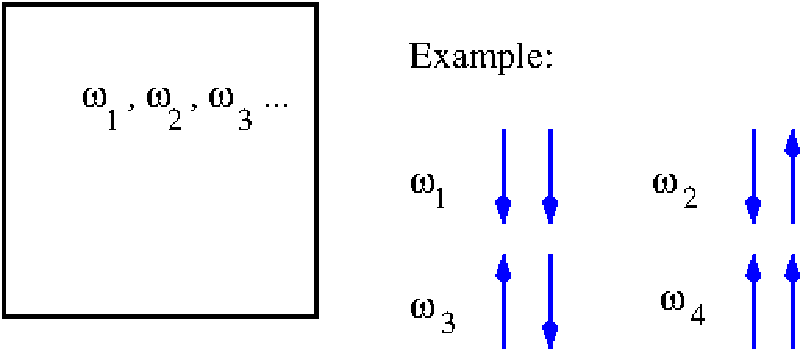
\includegraphics[width=0.7\textwidth]{figs/week03_spin-system.pdf}
\end{center}
To form the overall system $\Om_{\text{tot}}$ we now bring together the $R = 9$ replicas shown below.
We draw boxes around each replica to remind us that they are allowed to exchange only energy with each other, while the $N = 2$ spins are conserved in each replica.
We pick out one of these replicas (coloured red) to serve as the system \Om we will consider.
The other $8$ are the thermal reservoir $\Om_{\text{res}}$ that fixes the temperature of $\Om$.
\begin{center}
  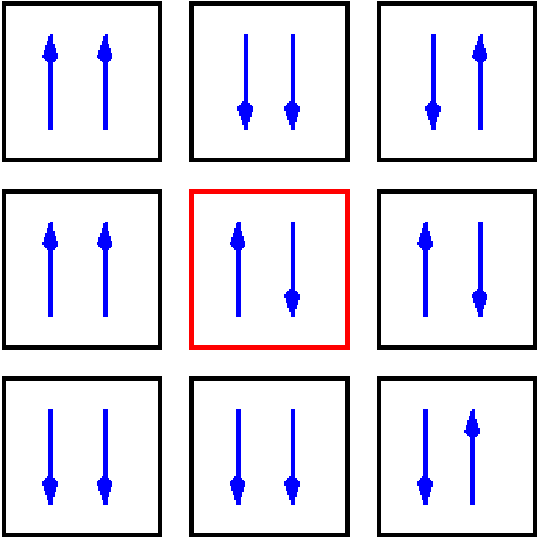
\includegraphics[width=0.7\textwidth]{figs/week03_spin-reservoir.pdf}
\end{center}

A convenient way to analyze the overall system of $R$ replicas, $\Om_{\text{tot}}$, is to define the \textbf{occupation number} $n_i$ to be the number of replicas that adopt the micro-state $\om_i \in \Om$ in any given micro-state of $\Om_{\text{tot}}$.
The index $i \in \left\{1, 2, \cdots, M\right\}$ runs over all $M$ micro-states of $\Om$.
In the example above, three of the replicas in the second figure have the micro-state $\om_1 = \downarrow\downarrow$, meaning $n_1 = 3$.
What are the occupation numbers $\left\{n_2, n_3, n_4\right\}$ for the other three $\om_i$ in the figures above?
Are all replicas are accounted for, $\sum_i n_i = R$?
\begin{mdframed}
  \ \\[50 pt]
\end{mdframed}
Normalizing the occupation number by $R$ gives us a well-defined \textit{occupation probability}, $p_i = n_i / R$ with $\sum_i p_i = 1$.
This $p_i$ is the probability that if we choose a replica at random it will be in micro-state $\om_i$.

Now let us consider conservation of energy, which continues to apply to the total energy $E_{\text{tot}}$ of the overall system $\Om_{\text{tot}}$.
We assume that each replica's energy $E_r$ is independent of all the other replicas.
This is guaranteed for the non-interacting systems we will focus on until week $10$, and also holds when interactions are allowed within each replica but not between different replicas.
The thermal contact between replicas allows $E_r$ to fluctuate (subject to conservation of $E_{\text{tot}}$), but there are only $M$ possible values $E_i$ it can have, corresponding to the $M$ micro-states $\om_i \in \Om$.
This allows us to rearrange a sum over replicas into a sum over the micro-states of $\Om$:
\begin{equation}
  \label{eq:canon_Etot}
  E_{\text{tot}} = \sum_{r = 1}^R E_r = \sum_{i = 1}^M n_i E_i,
\end{equation}
with the occupation number $n_i$ counting how many times micro-state $\om_i$ appears among the $R$ replicas.
We can assume that $R$ and $M$ are both finite, so we don't need to worry about rearranging infinite sums.
% ------------------------------------------------------------------



% ------------------------------------------------------------------
\subsubsection{Partition function}
Following Gibbs, we have already taken the thermal reservoir $\Om_{\text{res}}$ to consist of $R - 1$ replicas of the system of interest, $\Om$.
The next step is to further simplify the mathematics by assuming that the overall $R$-replica system $\Om_{\text{tot}}$ is fully specified by a fixed set of $M$ occupation numbers $\left\{n_i\right\}$.
From \eq{eq:canon_Etot}, we see that this ensures conservation of the total energy $E_{\text{tot}}$, and we can apply the micro-canonical tools we developed last week.
Recall our ultimate \textcolor{green}{goal} of showing that such details of the thermal reservoir are irrelevant to the system $\Om$.

Based on the conservation of $E_{\text{tot}}$, we want to determine the (intensive) temperature of $\Om_{\text{tot}}$, which fixes the temperature of the system of interest, $\Om$.
According to our work last week, to do this we first need to compute the overall number of micro-states $M_{\text{tot}}$ as a function of $E_{\text{tot}}$, from which we can derive the entropy and temperature since the system is in thermodynamic equilibrium.
From the fixed occupation numbers $n_i$, we already know how many times each micro-state $\om_i$ appears among the $R$ replicas.
To determine $M_{\text{tot}}$ we just need to count how many possible ways there are of distributing the $\left\{n_i\right\}$ micro-states among the $R$ replicas.

If we consider first the micro-state $\om_1$, the number of possible ways of distributing $n_1$ copies of this micro-states among the $R$ replicas is just the binomial coefficient
\begin{equation*}
  \binom{R}{n_1} = \frac{R!}{n_1! \; (R - n_1)!}.
\end{equation*}
Moving on to $\om_2$, we need to keep in mind that $n_1$ replicas have already been assigned micro-state $\om_1$, so there are only $R - n_1$ replicas left to choose from.
What is the resulting number of possible ways of distributing these $n_2$ micro-states?
\begin{mdframed}
  \ \\[50 pt]
\end{mdframed}
Repeating this process for all micro-states $\left\{\om_1, \om_2, \cdots, \om_M\right\}$, and recalling that $\left(R - \sum_i n_i \right)! = 0! = 1$, you should obtain a product that `telescopes' to
\begin{equation}
  \label{eq:telescoped}
  M_{\text{tot}} = \frac{R!}{n_1! \; n_2! \; \cdots \; n_M!}.
\end{equation}
From this we can see that the order in which we assign micro-states to replicas is irrelevant, since integer multiplication is commutative.

Thanks to thermodynamic equilibrium, the entropy of the micro-canonical overall system $\Om_{\text{tot}}$ is
\begin{equation*}
  S(E_{\text{tot}}) = \log M_{\text{tot}} = \log(R!) - \sum_{i = 1}^M \log(n_i!),
\end{equation*}
where the dependence on $E_{\text{tot}}$ enters through the occupation numbers via \eq{eq:canon_Etot}.
With $R \gg 1$ and $n_i \gg 1$ for all $i = 1, \cdots, M$, we can approximate each of these logarithms using the first two terms in \href{https://en.wikipedia.org/wiki/Stirling's_approximation}{Stirling's formula},
\begin{align*}
  \log(N!) & = N \log N - N + \cO(\log N) \approx N \log N - N &
  \mbox{for } N & \gg 1.
\end{align*}
Back in \eq{eq:CLT_states} we used the central limit theorem to derive a form of this approximation that included a leading term from the $\cO(\log N)$ we neglect here.
In order for \textit{every} occupation number to be large, $n_i \gg 1$, the number of replicas must be much larger than the number of micro-states of $\Om$, so that $R \gg M$.
As we have discussed before, the number of micro-states $M$ is typically a very large number, so we are formally considering truly enormous thermal reservoirs!
This enormity helps ensure that the detailed form of the reservoir will be irrelevant.

Applying the approximation above, what do you find for $S(E_{\text{tot}})$ in terms of $R$ and $n_i$?
What is the entropy in terms of the occupation probabilities $p_i = n_i / R$?
\begin{mdframed}
  $\displaystyle S(E_{\text{tot}}) = \log(R!) - \sum_{i = 1}^M \log(n_i!) \approx $ \\[100 pt]
\end{mdframed}

In your result, the dependence on $E_{\text{tot}}$ now enters through the occupation probabilities $p_i$.
In order to determine the temperature, we have to express $S(E_{\text{tot}})$ directly in terms of $E_{\text{tot}}$.
We do this by applying our knowledge from last week that thermodynamic equilibrium implies maximal entropy.

Following the same steps as last week, we maximize the entropy, including two Lagrange multipliers to account for the two constraints on the occupation probabilities:
\begin{align*}
  \sum_{i = 1}^M p_i & = 1 &
  \sum_{i = 1}^M n_i E_i & = R \sum_{i = 1}^M p_i E_i = E_{\text{tot}}.
\end{align*}
Writing everything in terms of occupation probabilities we therefore need to maximize the modified entropy
\begin{equation*}
  \Sbar = -R \sum_{i = 1}^M p_i \log p_i + \al\left(\sum_{i = 1}^M p_i - 1\right) - \be\left(R \sum_{i = 1}^M p_i E_i - E_{\text{tot}}\right).
\end{equation*}
(The sign of \be is irrelevant, and chosen for later convenience.)
What is the occupation probability $p_k$ that maximizes $\Sbar$?
\begin{mdframed}
  $\displaystyle 0 = \pderiv{\Sbar}{p_k} = $ \\[120 pt] % WARNING: FORMATTING BY HAND
\end{mdframed}

You should find a probability
\begin{equation}
  \label{eq:canon_prob}
  p_k = \frac{1}{Z} e^{-\be E_k},
\end{equation}
where we define $Z = \exp\left[1 - \frac{\al}{R}\right]$ to put the result in its traditional form.
In place of $\left\{\al, \be\right\}$, our free parameters are now $\left\{Z, \be\right\}$.
Still following last week's procedure, we need to fix these free parameters by demanding that the two constraints above are satisfied.
The first of these constraints is straightforward and produces an important result:
\begin{equation}
  \label{eq:part_func}
  1 = \sum_{i = 1}^M p_i = \frac{1}{Z} \sum_{i = 1}^M e^{-\be E_i} \qquad \implies \qquad Z(\be) = \sum_{i = 1}^M e^{-\be E_i}.
\end{equation}

\begin{shaded}
  Equation~\ref{eq:part_func} defines the canonical \textbf{partition function} $Z(\be)$, a fundamental quantity in the canonical ensemble, from which many other derived quantities can be obtained.
\end{shaded}

$Z(\be)$ still depends on the other as-yet-unknown free parameter $\be(E_{\text{tot}})$.
If we apply our second constraint, \eq{eq:canon_Etot}, we can relate \be to $E_{\text{tot}}$:
\begin{equation}
  \label{eq:canon_aveE}
  E_{\text{tot}} = R \sum_{i = 1}^M p_i E_i = \frac{R}{Z(\be)} \sum_{i = 1}^M E_i \; e^{-\be E_i} = R \frac{\sum_{i = 1}^M E_i \; e^{-\be E_i}}{\sum_{i = 1}^M e^{-\be E_i}}.
\end{equation}
This is a bit opaque, but will suffice for our goal of expressing the entropy in terms of $E_{\text{tot}}$.
Inserting \eq{eq:canon_prob} for $p_i$ into your earlier result for the entropy, what do you obtain upon applying Eqs.~\ref{eq:part_func} and \ref{eq:canon_aveE}?
\begin{mdframed}
  $\displaystyle S(E_{\text{tot}}) = -R \sum_{i = 1}^M p_i \log p_i = $ \\[100 pt]
\end{mdframed}
There is a pleasant simplification when we take the derivative to determine the temperature.
Defining $\be' = \pderiv{}{E_{\text{tot}}} \be(E_{\text{tot}})$, we have
\begin{equation*}
  \frac{1}{T} = \pderiv{}{E_{\text{tot}}} S(E_{\text{tot}}) = \pderiv{}{E_{\text{tot}}} \left[E_{\text{tot}} \be + R\log Z(\be)\right] = \be + E_{\text{tot}} \be' + R \frac{1}{Z} \pderiv{Z(\be)}{\be} \be' .
\end{equation*}
Using \eq{eq:canon_aveE} we can recognize
\begin{equation*}
  \frac{1}{Z} \pderiv{Z(\be)}{\be} = \frac{1}{Z} \pderiv{}{\be} \sum_{i = 1}^M e^{-\be E_i} = -\frac{1}{Z} \sum_{i = 1}^M E_i \; e^{-\be E_i} = -\frac{E_{\text{tot}}}{R},
\end{equation*}
so that we don't need to figure out the explicit form of $\be'$:
\begin{equation}
  \label{eq:beta}
  \frac{1}{T} = \be + E_{\text{tot}} \be' - E_{\text{tot}} \be' = \be .
\end{equation}

What's truly remarkable about \eq{eq:beta} is that all the details of the thermal reservoir have vanished---there is no reference to the $R$ replicas or any extensive quantity such as $E_{\text{tot}}$.
This is \textcolor{green}{the goal} we have been pursuing since the start of the notes for this week!
The large thermal reservoir is still present to fix the temperature $T$ characterizing the canonical system $\Om$, but beyond that nothing about it is relevant---or even knowable in the canonical approach.
Every aspect of \Om can now be specified in terms of the fixed temperature $T$ and conserved particle number $N$, starting with the parameter $\be = 1 / T$.

In particular, the partition function from \eq{eq:part_func} is simply
\begin{equation}
  Z(T) = \sum_{i = 1}^M e^{-E_i / T}.
\end{equation}
and together with \be specifies the probabilities
\begin{equation}
  p_i = \frac{1}{Z} e^{-E_i / T}
\end{equation}
from \eq{eq:canon_prob}.
This $p_i$ is now the probability---in thermodynamic equilibrium---that \Om adopts micro-state $\om_i$ with (non-conserved) internal energy $E_i$.
As we might have expected based on last week's look at the micro-canonical ensemble, all micro-statse with the same energy have the same probability in thermodynamic equilibrium.
% ------------------------------------------------------------------



% ------------------------------------------------------------------
\subsection{Internal energy, entropy and heat capacity}
Now that the temperature of the system \Om is fixed, its internal energy is no longer conserved, and can fluctuate by exchanging energy with the thermal reservoir.
Although the internal energy fluctuates, its expectation value $\vev{E}$ is a derived quantity of interest, which can be defined in the usual way for the probability space of the canonical ensemble:
\begin{equation*}
  \vev{E}\!(T) = \sum_{i = 1}^M E_i \; p_i = \frac{1}{Z} \sum_{i = 1}^M E_i e^{-\be E_i}.
\end{equation*}
Here we have explicitly noted the temperature-dependence of $\vev{E}$, and also freely interchanged $\be = 1 / T$, in part because the last expression may \TODO{...}


\TODO{Being written...}
% ------------------------------------------------------------------



% ------------------------------------------------------------------
\newpage % TODO: Placeholder...
\subsection{Helmholtz free energy}
\TODO{Being written...}
% ------------------------------------------------------------------



% ------------------------------------------------------------------
\newpage % TODO: Placeholder...
\subsection{Distinguishable Spins}
\TODO{Being written...}
% ------------------------------------------------------------------



% ------------------------------------------------------------------
\newpage % TODO: Placeholder...
\subsection{Indistinguishable Spins}
\TODO{Being written...}
% ------------------------------------------------------------------
